\section{Evaluation}
\label{sec:res}

%\ameer{Hasan: Describe how the random programs generator works and used and how the cost model was trained}\newline
%\jenny{Can we show the total number of cost model evaluations and the min cost found from each method we evaluate?}


To evaluate ProTuner we built it on top of Halide in C++. We run ProTuner on AWS m5.8xlarge instances. These instances run Intel Xeon Platinum 8259CL processors with 16 physical cores with, 128 GB RAM and 100 GB SSD storage. AWS often provides different CPUs for different instances even if they are from the same type (\textit{e.g}., m5.8xlarge can have Intel Xeon Platinum 8259CL processors or Intel Xeon Platinum 8175M processors). To minimize variance between runs we run all our results on the same instance, during the same time of the day, when it is night time in the time zone and after turning off hyperthreading. Details for reproducing our results are available in the appendix. The code will also be open-sourced for further research and development.

We set the timeout limit for picking a new root in the MCTS to 30 seconds. We also explore reducing that to one second and include real execution time measurements. We use 16 MCTS (one greedy, 15 standard) that run in parallel and synchronize every timeout for picking a new root. For an apples-to-apples comparison, we also run 16 beam searches in parallel. We use the open-sourced code of Halide's beam search algorithm with the artifacts published by the original authors with the same configuration of provided in~\cite{adams2019learning} with a beam size of 32 and five passes (iterations of beam search). We also compared our results to a greedy auto-scheduler (beam size of 1), the default scheduler on Halide's master branch, and random search. Random search does not use the cost model. It runs for ten minutes and outputs the program with the best real execution time it found. The other algorithms run with three different seeds and the best performing schedule found by each algorithm is reported. 

We auto-scheduled a suit of 16 real applications. These applications range from matrix multiplications to various blurs, convolutions and interpolations, to full implementation of ResNet50~\cite{he2016deep}. These applications were taken from the baseline beam search work we compare against and are available on the Halide repository. We experimented with multiple MCTS configurations as shown in Table~\ref{tab:dse}. We mainly experimented with different timeouts for determining a new root while running the MCTS algorithm, the expansion formula that determines, which child in the tree gets expanded and integrating real execution time measurements during the search. 

\begin{figure*}[!t]
    \centering
    \begin{subfigure}[t]{\textwidth}
        \centering
        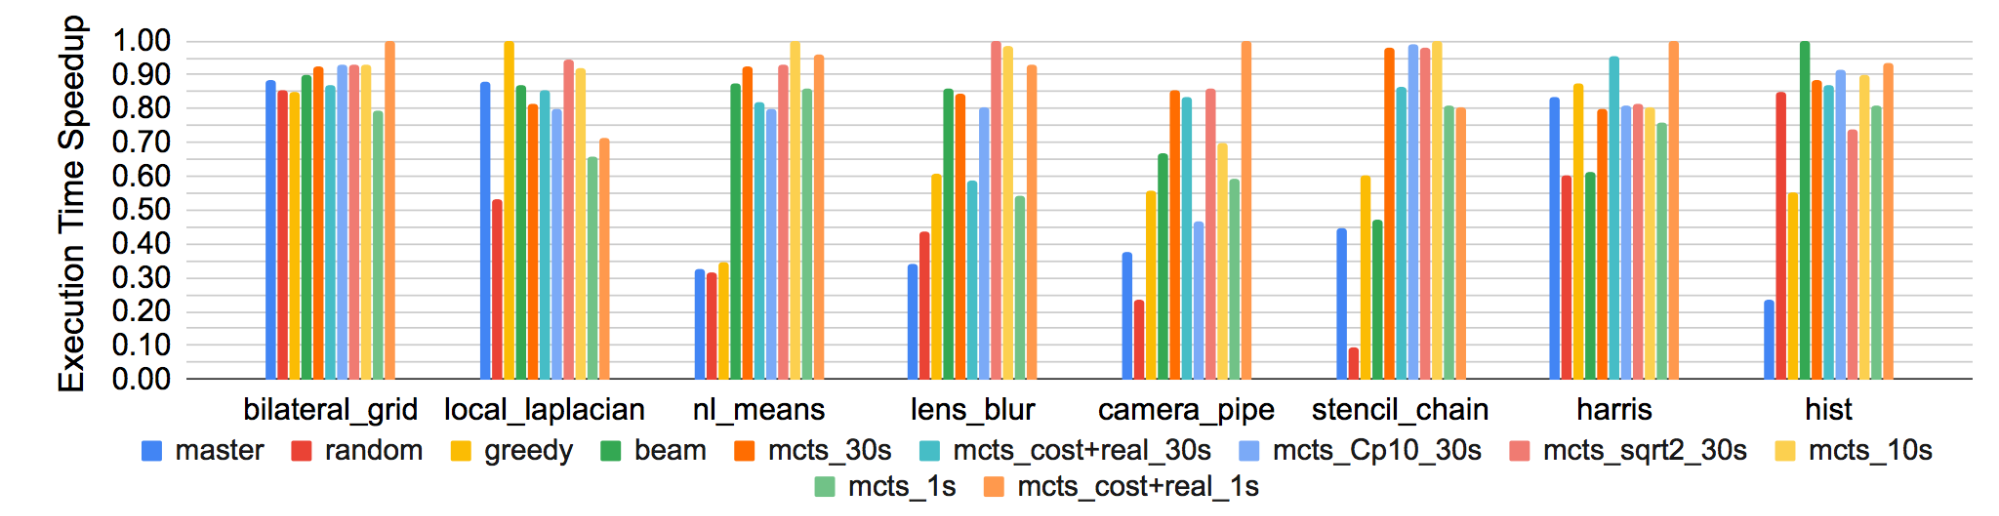
\includegraphics[trim={0cm 2.9cm 0cm 0cm},clip,width=\textwidth]{figures/perf1.png}
    \end{subfigure}
    \begin{subfigure}[t]{\textwidth}
        \centering
        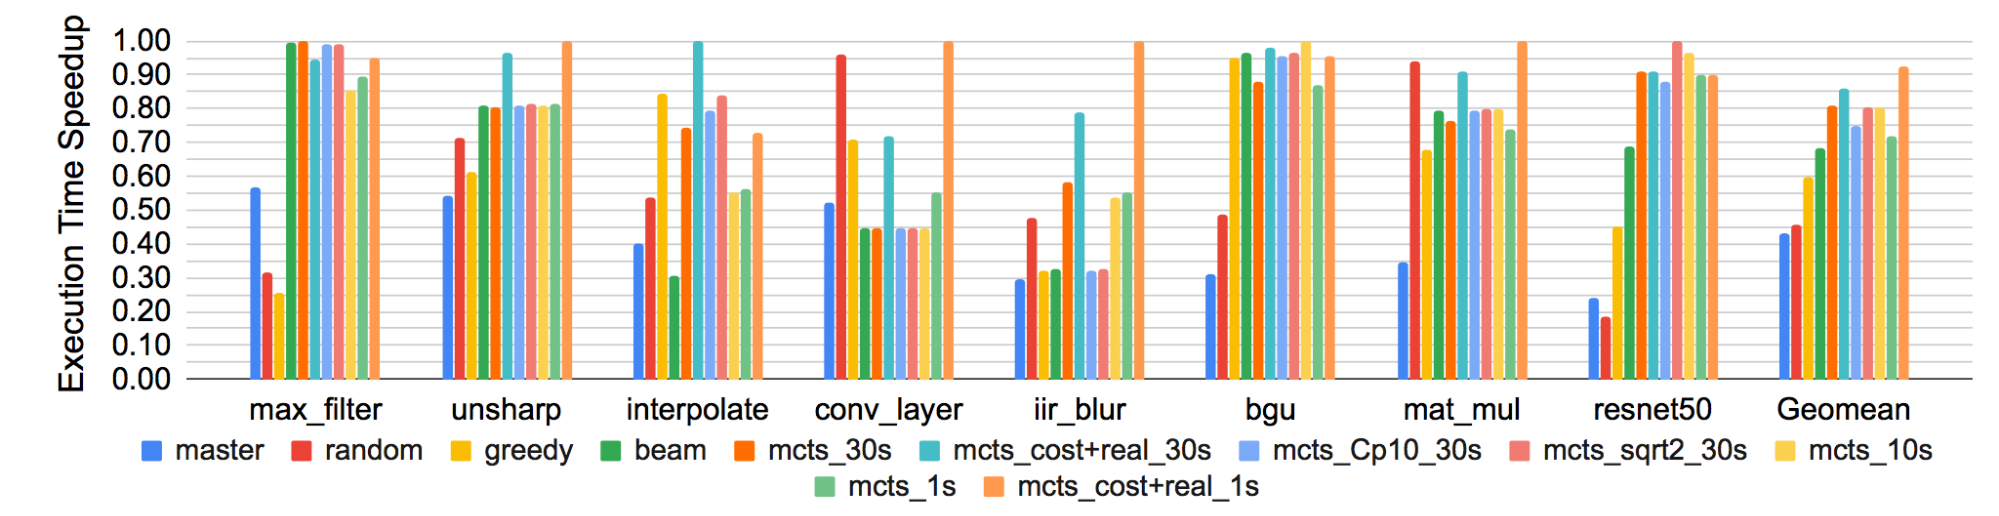
\includegraphics[width=\textwidth]{figures/perf2.png}
    \end{subfigure}
    \caption{The minimum execution time found by every algorithm normalized to the best execution time found by all the algorithms on a suite of 16 real benchmarks.}
    \label{fig:perf}
\end{figure*}
\subsection{Cost}
Figure~\ref{fig:cost} shows the minimum costs found by our MCTS algorithms compared to random, greedy, and beam search. The costs are normalized to the best cost found by all the algorithms. The cost of ResNet50 is omitted because the application includes multiple stages, each stage is auto-scheduled separately (with costs in different ranges) and later the stages are merged back to form the final application.
We observe that our MCTS outperforms beam, greedy, random search cost-wise in geometric mean, in all the MCTS configurations. This means that with a cost model that has 100\% accuracy, our MCTS achieves better performance than that of beam, greedy, and random search. \texttt{mcts\_Cp10\_30s} costs outperform the costs of beam search in all the benchmarks. \texttt{mct\_30s} outperforms beam search in all the benchmarks except \texttt{iir\_blur}, in which it achieves costs 4.5\% worse than beam search. \texttt{mct\_10s} outperforms beam search in all the benchmarks except \texttt{nl\_means}, and \texttt{iir\_blur} in which it achieves costs 8.9\% and 1.1\% worse than beam search, respectively. \texttt{mcts\_sqrt2\_30s} outperforms beam search in all the benchmarks except \texttt{nl\_means} and \texttt{iir\_blur}, which achieve  costs 5.2\% and 2.4\% worse than beam search, respectively. \texttt{mcts\_cost+real\_30s} and \texttt{mcts\_cost+real\_1s} achieve the worst geometric mean cost among the MCTS algorithms. This means that they found schedules with better execution times but at higher costs. 

\subsection{Execution Time}
Figure~\ref{fig:perf} shows the minimum execution time each algorithm found normalized to the best execution time found by all the algorithms. Note that the scale in costs and execution times is different.  Similar to the costs, in geometric mean, all the MCTS algorithms outperform beam search ($1.06\times$-$1.36\times$), even \texttt{mcts\_1s}, which gives one second for each MCTS iteration. our biggest execution time improvement is observed in \texttt{interpolate} where we achieve $1.8\times$-$3.25\times$ better performance in the different MCTS algorithms. 

As expected,  \texttt{mcts\_cost+real\_30s} and \texttt{mcts\_cost+real\_1s} achieve the best performance in geometric mean. This is despite not achieving the best geometric mean in costs. This shows that real execution time measurement is effective. Interestingly, \texttt{mcts\_cost+real\_1s} achieves better performance than \texttt{mcts\_cost+real\_30s}. The first is less likely to overfit to the cost model than the second. A clear example can be seen in \texttt{conv\_layer}, which is the smallest benchmark. While both \texttt{mcts\_cost+real\_1s} and \texttt{mcts\_cost+real\_30s} outperform the other MCTS algorithms, the first achieves better performance as it stops evaluating the cost model earlier and hence it is less likely to overfit to the cost model, especially on smaller benchmarks.


%Note that \texttt{mcts\_cost+real\_30s} achieves the same performance as \texttt{mcts\_30s} on applications that the cost model predicts with an accuracy higher than that of the other applications in which \texttt{mcts\_cost+real\_30s} achieves better performance than \texttt{mcts\_30s}. 
% \begin{figure*}[!t]
%     \centering
%     \begin{subfigure}[t]{\textwidth}
%         \centering
%         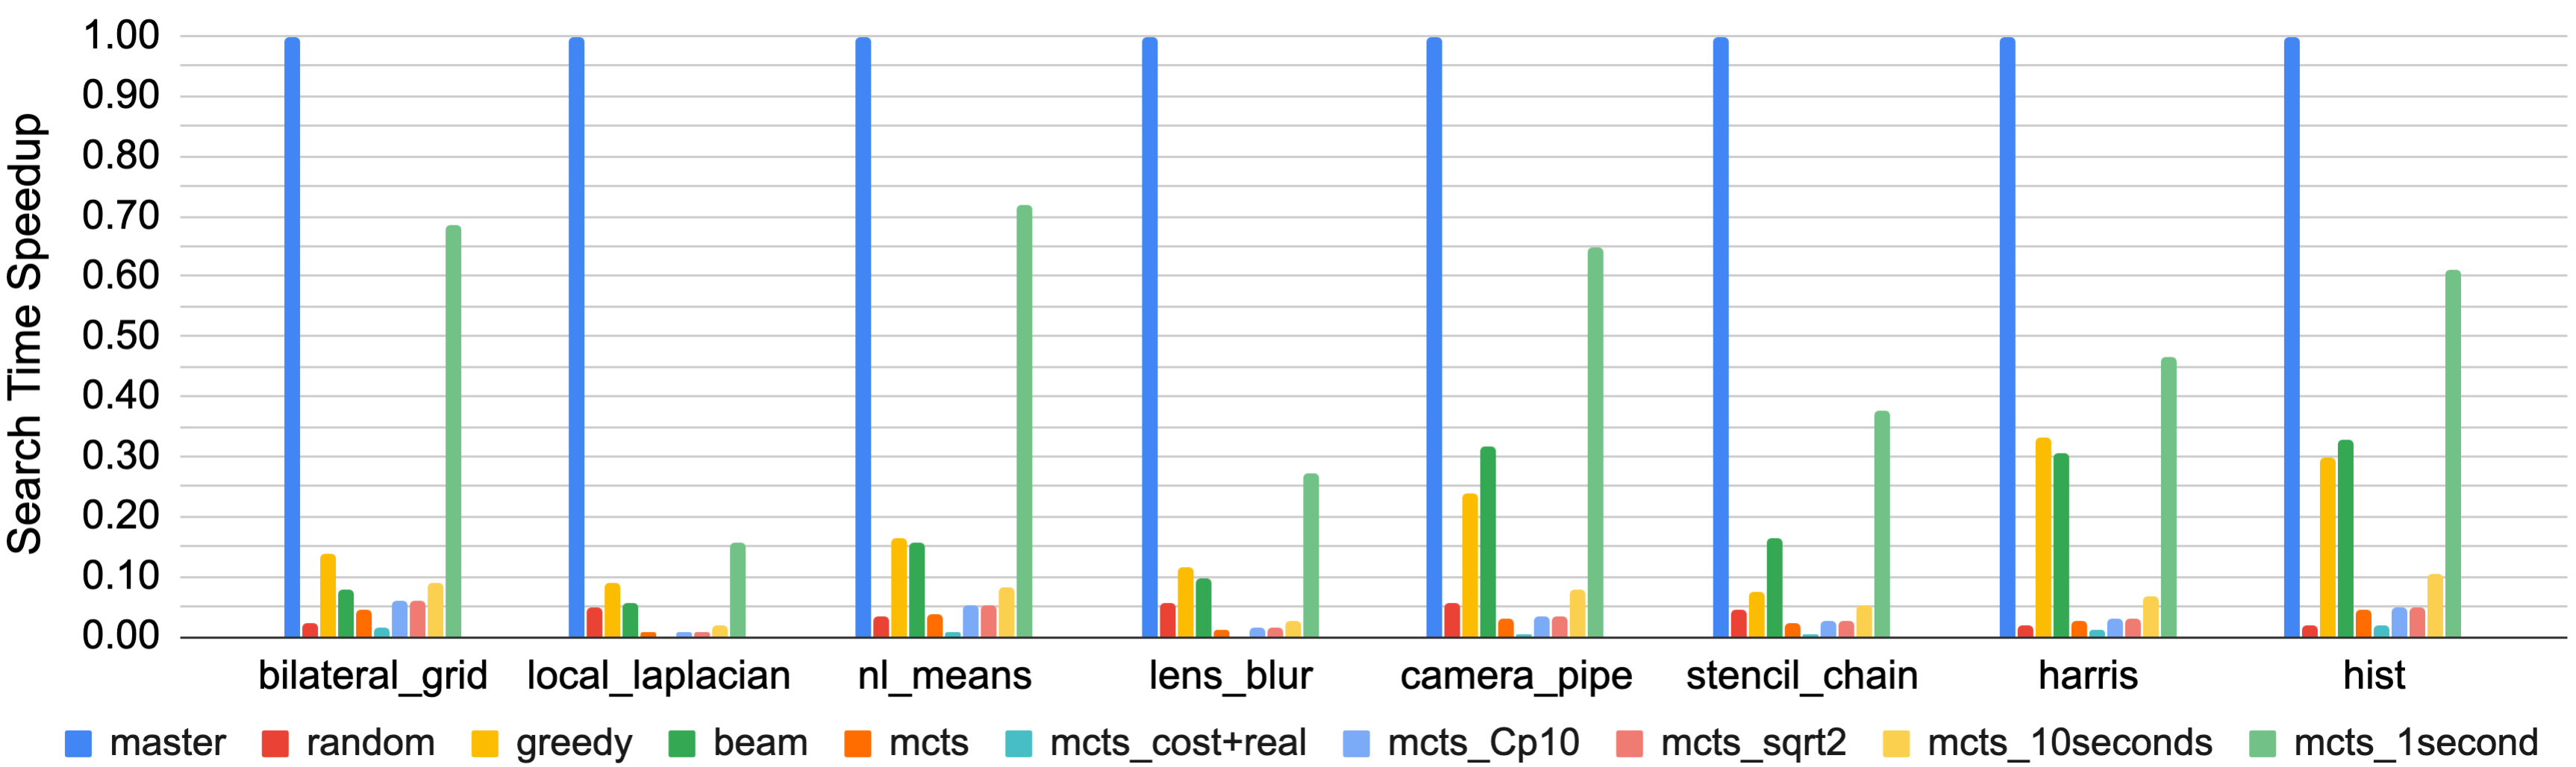
\includegraphics[trim={0cm 1.5cm 0cm 0cm},clip,width=\textwidth]{figures/runtime1.png}
%     \end{subfigure}
%     \begin{subfigure}[t]{\textwidth}
%         \centering
%         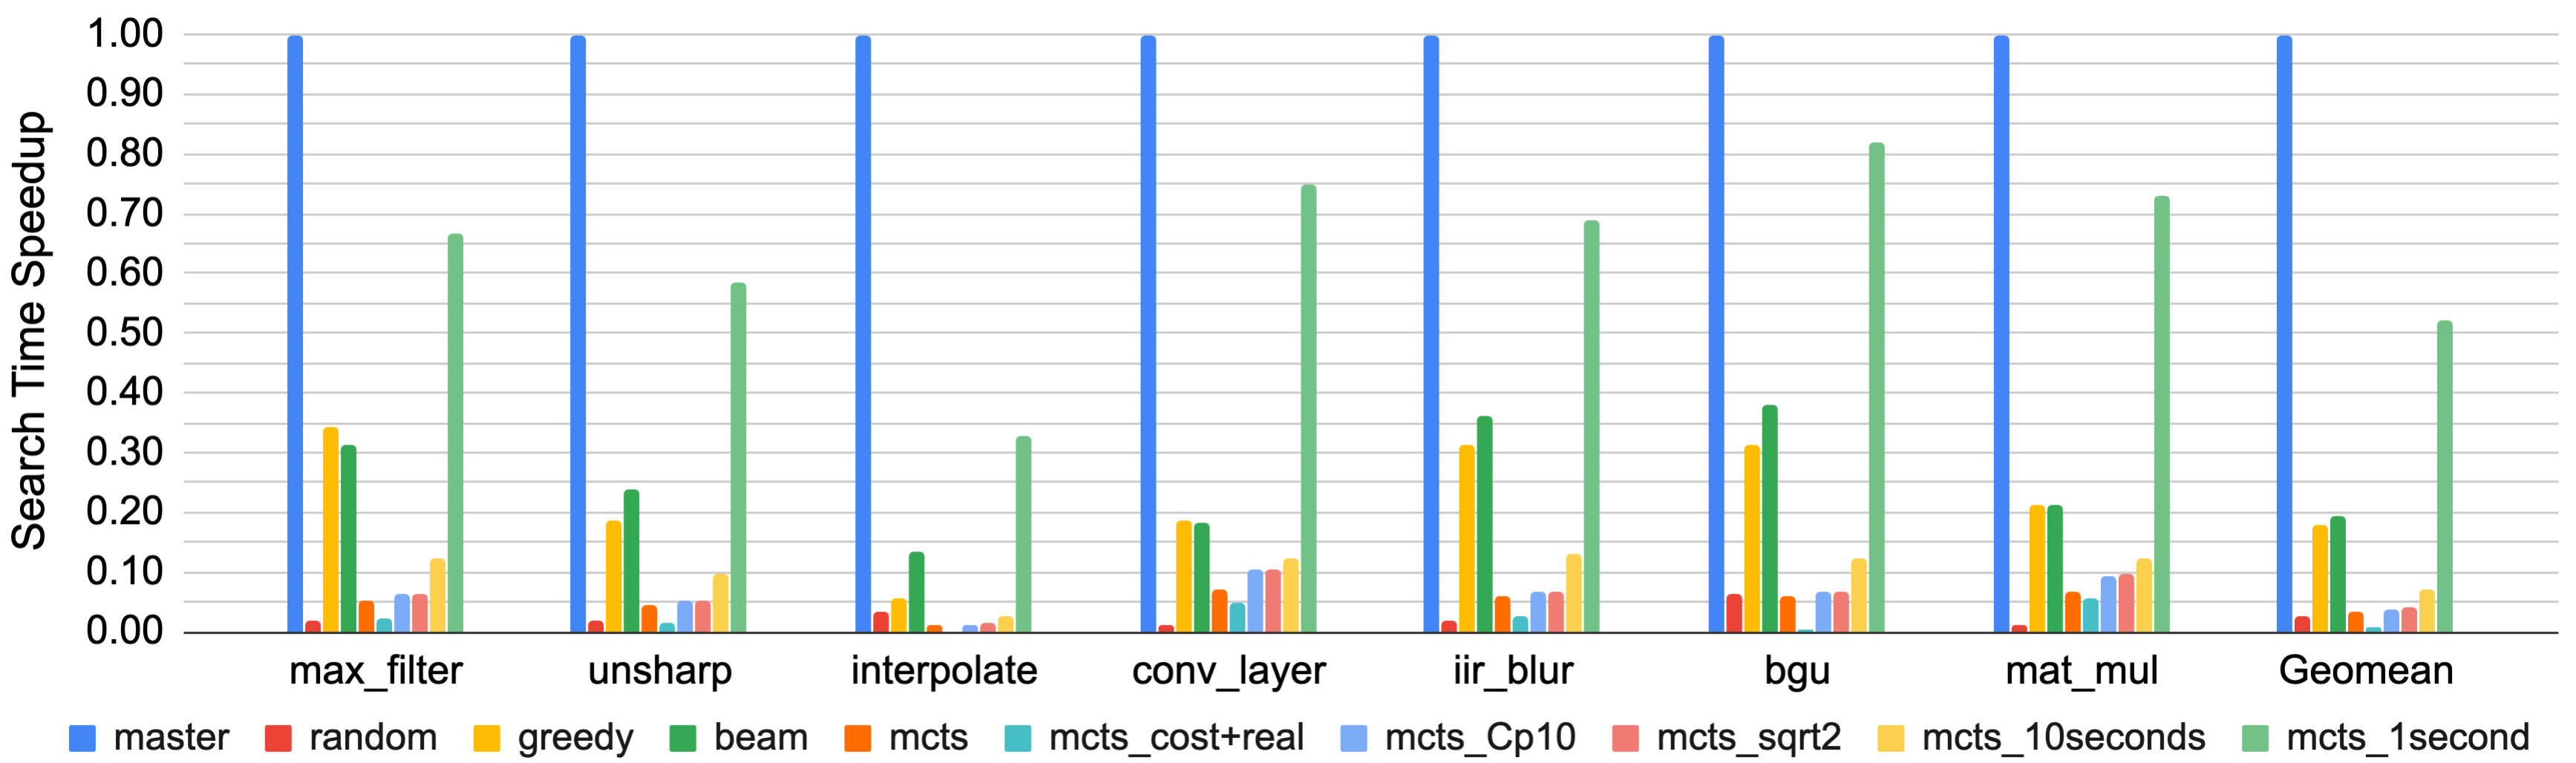
\includegraphics[width=\textwidth]{figures/runtime2.png}
%     \end{subfigure}
%     \caption{The average search time found by every algorithm normalized to the fastest search algorithm on a suite of 16 real benchmarks.}
%     \label{fig:runtime}
% \end{figure*}

We observe that \texttt{mcts\_10s} achieves similar performance to \texttt{mcts\_30s} and \texttt{mcts\_sqrt2\_30s}, and better performance than \texttt{mcts\_Cp10\_30s} in geometric mean. This means that 10 seconds per MCTS iteration is sufficient for our benchmarks. Adding more time might be useful for large benchmarks but can be harmful to smaller benchmarks where the MCTS might overfit to the cost model. An ideal configuration should consider the size of the application when setting the MCTS parameters.

%We observe that \texttt{mcts\_1s} outperforms \texttt{mcts\_10s} in geometric mean. This is because \texttt{mcts\_1s} is less likely to overfit to the cost model in smaller applications such as \texttt{conv\_layer}. In larger applications, such as \texttt{lens\_blur}, \texttt{mcts\_10s} outperforms \texttt{mcts\_1s} as longer iterations allow the MCTS to find better costs in larger applications.
\begin{figure*}
    \centering
    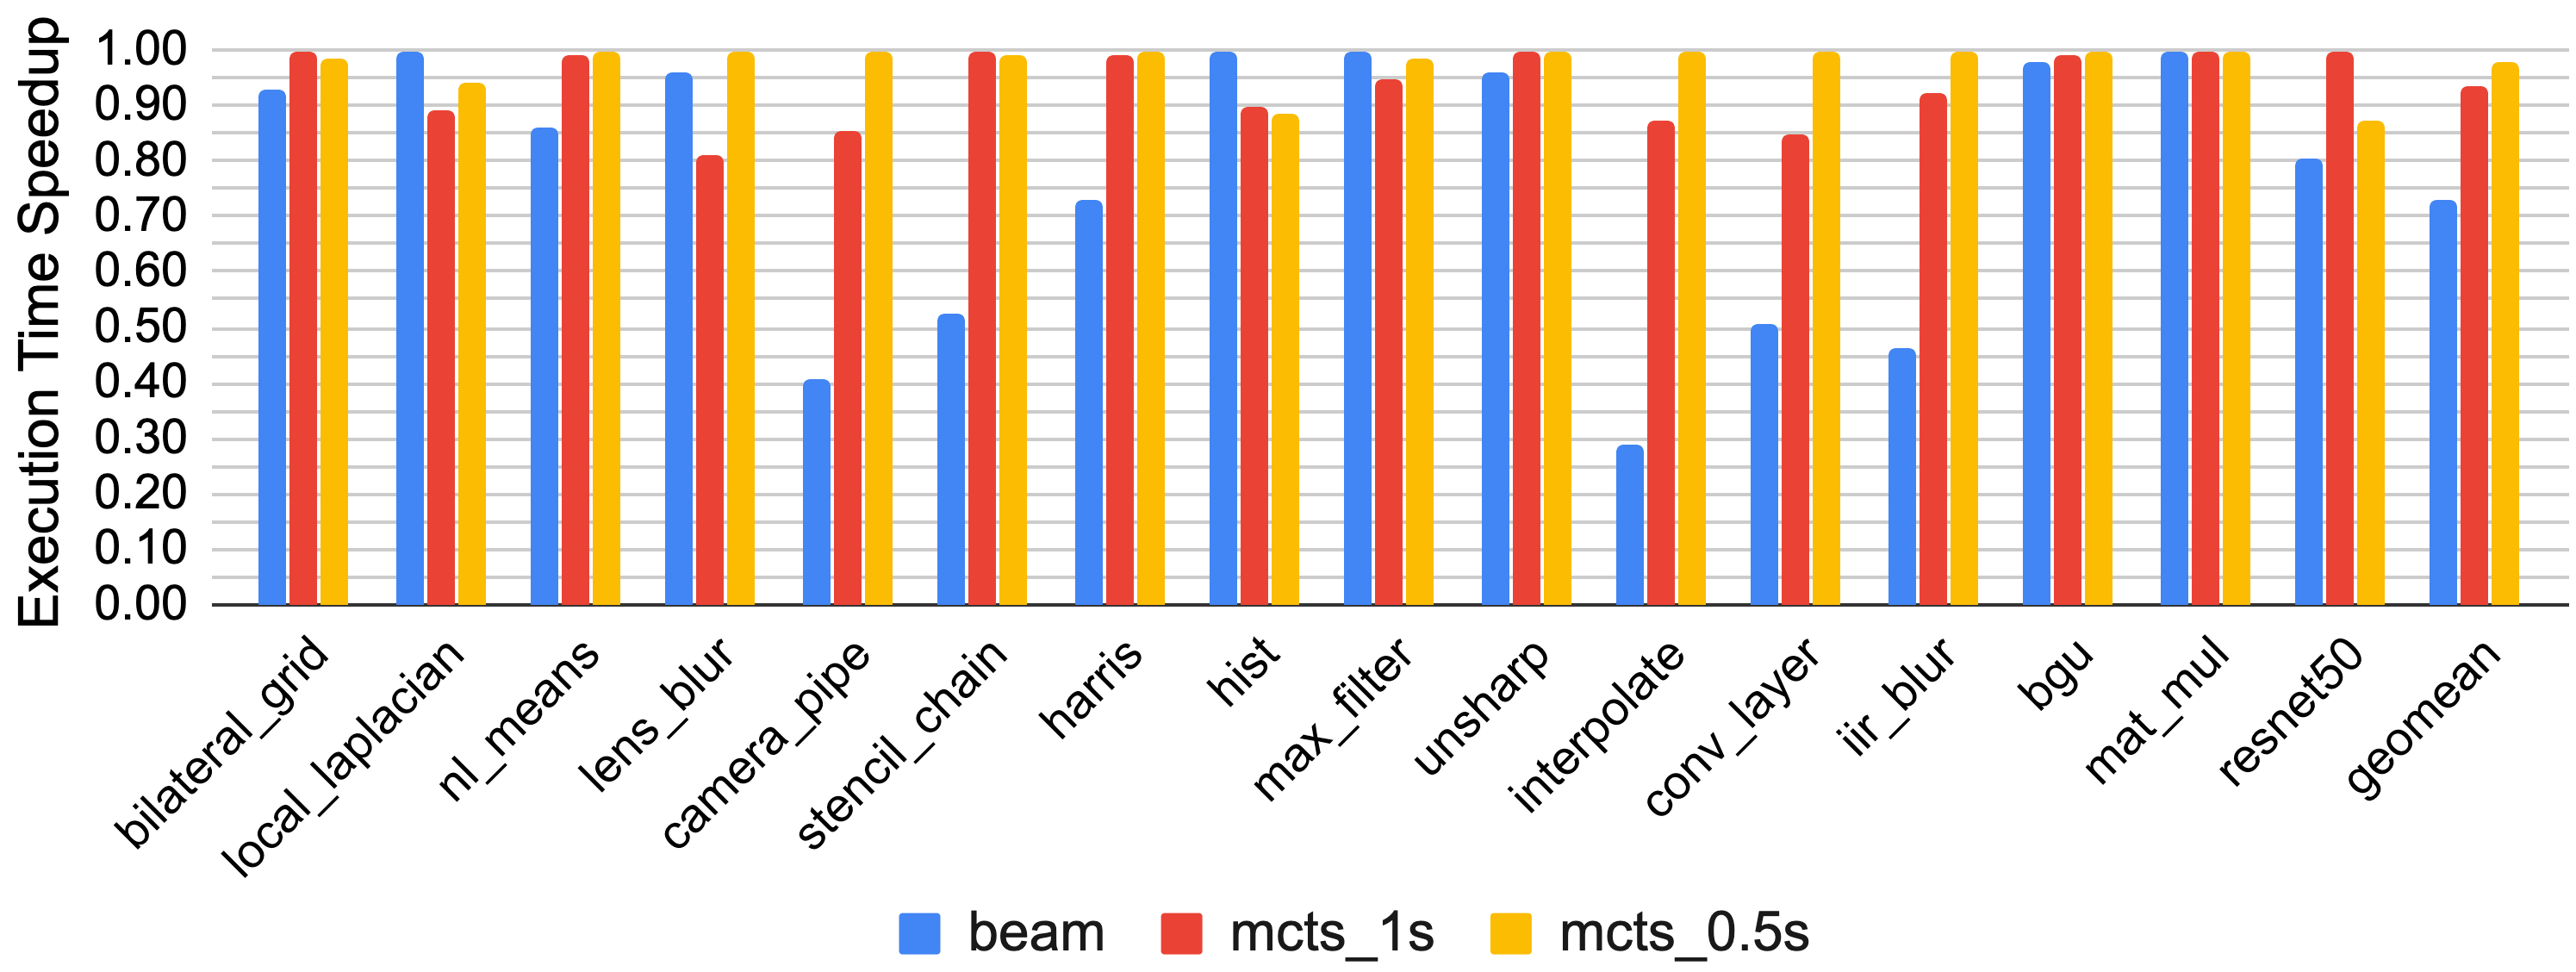
\includegraphics[width=\textwidth]{figures/autotune2.png}
    \caption{Execution time speedup normalized to the best execution time using beam search, \texttt{mcts\_1s}, and \texttt{mcts\_0.5s} with autotuning on a suite of 16 real benchmarks. Each algorithm is rerun with a different seed until a timeout of 15 minutes is reached and the bests performance found by each algorithm is reported.}
    \label{fig:autotune}
\end{figure*}

%Interestingly, the second best performing is \texttt{mcts\_sqrt2\_30s}, which uses the original UCB formula, and encourages much more exploration than the other MCTS algorithms resulting in more resilience to noise in the costs. We used $C_p = \frac{1}{\sqrt{2}}$ as suggested in~\cite{kocsis2006improved}, which showed that it works well with rewards in range $[0,1]$ as it satisfies the Hoeffding inequality. We observe that for \texttt{mcts\_sqrt2\_30s} the cost and execution time behave similarly except for \texttt{nl\_means}, \texttt{hist}, and \texttt{iir\_blur}. In the first, \texttt{mcts\_sqrt2\_30s} achieves worse cost but better execution time as it is more resilient to noise in the cost. In the later two, \texttt{mcts\_sqrt2\_30s} achieves better cost but worse execution time because the cost model generates inaccurate costs that allow random search to outperform some of the MCTS algorithms, beam search and greedy search. Our biggest execution time improvement is observed in \texttt{interpolate} where we achieve $1.9\times$-$3.5\times$ better performance in the different MCTS algorithms. 

\subsection{Search Time}
Our MCTS algorithms with the cost model schedule programs in seconds to minutes. Among all the benchmarks, the average auto-scheduling time of \texttt{mcts\_1s}, \texttt{mcts\_10s}, and \texttt{mcts\_30s} are 31, 155, 422 seconds respectively. This includes the time to compile the search code, the search time, and the time to compile and benchmark the applications. In smaller applications, such as~\texttt{conv\_layer} and~\texttt{mat\_mul}, this time is dominated by the compilation and benchmarking time. For larger applications, this time is dominated by the search time. Our performance analysis shows that most of the search time (88\%) is spent during the generation of new children (schedules) in the simulation phase and only 7.5\% of the time is spent in the cost evaluation. However, our standard MCTS simulation needs a single randomly generated child. The rest of the children are generated but not used. Therefore we see a potential for $8\times$ speedup in the search time of MCTS, which we seek to implement in future work.

For \texttt{mcts\_cost+real\_1s} and \texttt{mcts\_cost+real\_30s} the average auto-scheduling time is 23 and 35 minutes, respectively. Most benchmarks require roughly $3\times$ more time to auto-schedule with real execution time measurement when the MCTS iteration is set to 30 seconds. This time mostly consumed in the forked children processes that compile and evaluate the candidates of potential next roots serially. While it might seem to be inefficient to do this serially, we chose do it that way to avoid interference between threads during execution time measurement. 

% Figure~\ref{fig:runtime} shows the average time it took to run each search algorithm normalized to the fastest search time which happens to be the master baseline in all the benchmarks. Note that the master baseline mainly uses heuristics to generate the schedules rather than run a search algorithm with a learned cost model. While the master baseline is the fastest, its generated programs perform the worst with . The second fastest algorithm ($1.9\times$ slower than master in geometric mean) is \texttt{mcts\_1s}. \texttt{mcts\_1s} is $2.7\times$ ($1.52\times-8.52\times$) faster and $3.1\times$ ($1.4\times-7.96\times$) more tuning efficient\footnote{Tuning efficiency is computed as the execution time improvement divided by the search time.} than beam search in geometric mean. This means that \texttt{mcts\_1s} is better fit for autotuning than beam search. The other MCTS algorithms that use 30 seconds per iteration (\texttt{mcts\_30s},\texttt{mcts\_Cp10\_30s}, and \texttt{mcts\_sqrt2\_30s}) are on average $5.2\times$ slower than beam search and $2.67\times$ slower for \texttt{mcts\_10s}. 


\subsection{Autotuning with Limited Time Budget}
Figure~\ref{fig:autotune} shows the autotuning performance comparison between beam search and MCTS. We limit the autotuning time to 15 minutes for each application. This time includes the compilation and execution time of the benchmarks as well as the search time. The execution time of the generated program is normalized to the best execution time found by beam search and MCTS. For time efficiency we use \texttt{mcts\_1s}. We further explored using half a second per MCTS iteration (\texttt{mcts\_0.5s}), which allows for more real execution time measurements during autotuning. Each algorithm is rerun with a different seed until the timeout of 15 minutes is reached and the best performance found by each algorithm is reported. \texttt{mcts\_0.5s} achieves the best overall performance and outperforms beam search by up to $3.43\times$ and by $1.35\times$ in geometric mean, in the same time budget. \texttt{mcts\_1s} also outperforms beam search by up to $3\times$ and by $1.29\times$ in geometric mean in the same time budget. This is mainly due to more accurate scheduling decisions derived by meaningful costs of fully scheduled programs rather than incomplete programs. 
% We compared the schedules generated by ProTuner against those generated by Halide's existing default scheduler, as well as against a greedy autoscheduler and a beam autoscheduler which were both proposed in~\cite{adams2019learning}. Finally, we compared against schedules that were handwritten by experts, also found within the official Halide repo.

% AlphaHalide, the greedy autoscheduler, and the beam autoscheduler all evaluate the throughput of possible schedules with a cost model implemented as a simple feed-forward neural network, as described in~\cite{}. However, we found that the weights of this neural network found in the Halide repo were not very accurate for the our testing setup. Therefore, we retrained the weights on samples of randomly generated Halide pipelines and schedules using the same process described in~\cite{}. \textcolor{red}{Is more detail necessary here? Is it OK for us to use the weights trained on the benchmarks themselves?}

% We schedule and run our workloads on a server class computer: a 32-core Intel Xeon E5-2667V2 (3.3 GHz) CPUs with 256 GB DDR3 RAM.

% We run an ensemble of 20 MCTS in parallel. We force the MCTSes to make a scheduling decision every 10,000 simulations or 30 seconds (whichever occurs first). However, we also test how well the MCTSes do when they have no time limitation at all, and are only limited by the number of simulations. For the beam search and greedy autoschedulers, we use the parameters given in~\cite{}. Therefore, we set the beam size to 32, and the ``random dropout'' of proposed states to zero (i.e. no dropout).

% All our results can be reproduced by running \texttt{./generate\_all\_apps\_results} script available in our Github repo. The methodology is summarized in Table~\ref{tab:methodology}. \textcolor{red}{Hasan: I still need to fill this out...}

% \begin{table}[!t]
% \centering
% \begin{tabular}{|l|c|l|c|}
% \hline
% \textbf{Node} & \begin{tabular}[c]{@{}c@{}}2$\times$Intel Xeon\\ E5-2667V2\end{tabular} & \textbf{# Trees} & 20 \\ \hline
% \textbf{L1/L2/L3} & \begin{tabular}[c]{@{}c@{}}32KB/256KB\\ ./25MB\end{tabular} & \textbf{\begin{tabular}[c]{@{}l@{}}Max simulations\\ in each iteration\end{tabular}} & 10,000 \\ \hline
% \textbf{Memory} & 256 GB & \textbf{\begin{tabular}[c]{@{}l@{}}Max seconds \\ in each iteration\end{tabular}} & 30 \\ \hline
% \end{tabular}
% \caption{The Methodology and parameters used in our evaluation.}
% \label{tab:methodology}
% \end{table}

% \begin{table*}[!t]
% \centering
% \begin{tabular}{|c|c|c|c|c|}
% \hline
% \textbf{Experiment} & \textbf{Value Function} & \textbf{Greediness ($p$)} & \textbf{Next Root} & \textbf{Weights} \\ \hline
% \textbf{1} & Average cost & 0 & Best & Trained on random \\ \hline
% \textbf{2} & Average cost & 0.5 & Best & Trained on random \\ \hline
% \textbf{3} & Average cost & 1.0 & Best & Trained on random \\ \hline
% 4 & Average cost & 0 & Average & Trained on random \\ \hline
% \textbf{5} & Average wins & 0 & Best & Trained on random \\ \hline
% \textbf{6} & Average cost & 0 & Best & Trained on benchmarks \\ \hline
% \end{tabular}
% \caption{The experiments we run. We experiment with introducing greediness in simulation with probability $p$, different value functions, weights and how the determine the next root.}
% \label{tab:exps}
% \end{table*}
% We run six experiments described in Table~\ref{tab:exps}. The baseline uses MCTSes that use the average cost to search but the best cost to determine the next root. We then experiment with introducing different value functions, greediness, root picking strategy, and weights. \textcolor{red}{What do we mean by different greediness here?}

% When MCTS is not bounded by any time limitations, it performs quite well, beating all the other autoschedulers tested as well as the handcoded expert schedules. AlphaHalide achieves a geometric mean speedup over the default halide scheduler of $2.2\times$, while the greedy autoscheduler achieves only $1.1\times$ and the beam autoscheduler achieves $1.5\times$. These results are summarized in Fig.~\ref{fig:unbounded}. \textcolor{red}{Hasan: Should we put the compilation time here as well for the unbounded times? Or should we put the number of samples evaluated like Jenny suggests?}

% \begin{figure*}[h]
% \begin{subfigure}{\textwidth}
%   \centering
%   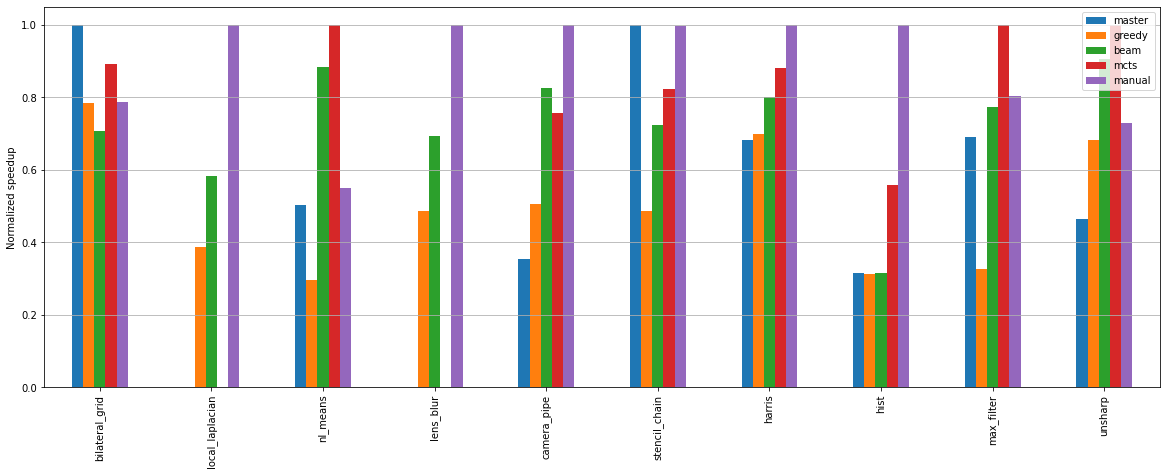
\includegraphics[width=.8\linewidth]{figures/unbounded1.png}
% \end{subfigure}

% \begin{subfigure}{\textwidth}
%   \centering
%   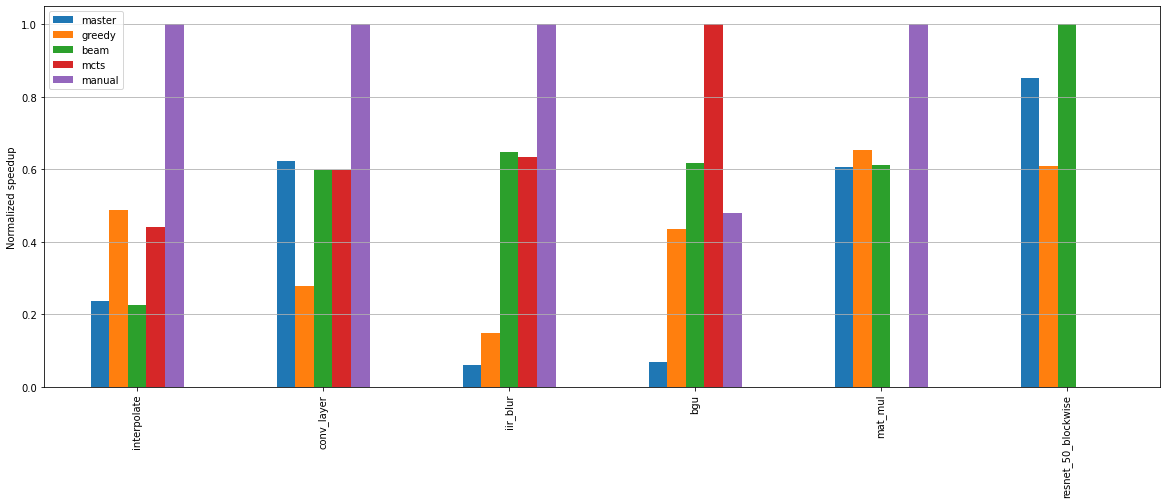
\includegraphics[width=.8\linewidth]{figures/unbounded2.png}
% \end{subfigure}
% \caption{Results when MCTS scheduling decisions are not limited by time.}
% \label{fig:unbounded}
% \end{figure*}

% On the other hand, when we force AlphaHalide to make a scheduling decision every 30 seconds at most, MCTS's performance drops considerably, falling to a geometric mean of only $1.2\times$ over the default autoscheduler, which is less than the greedy and beam autoschedulers, as seen in Fig.~\ref{fig:bounded}.

% \begin{figure*}[h]
% \begin{subfigure}{\textwidth}
%   \centering
%   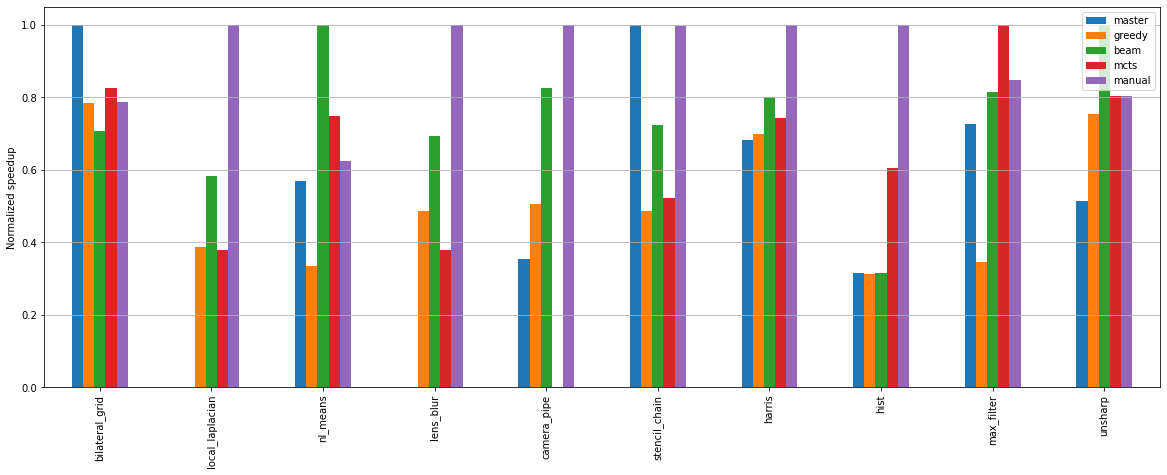
\includegraphics[width=.8\linewidth]{figures/bounded1.png}
% \end{subfigure}

% \begin{subfigure}{\textwidth}
%   \centering
%   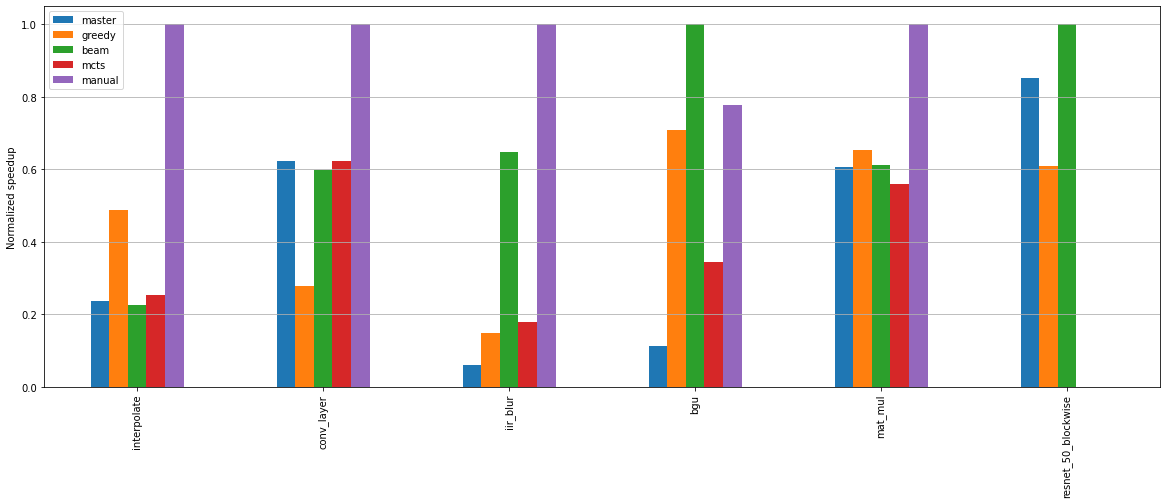
\includegraphics[width=.8\linewidth]{figures/bounded2.png}
% \end{subfigure}
% \caption{Results when MCTS scheduling decisions must be made every 30 seconds at most.}
% \label{fig:bounded}
% \end{figure*}

% \ameer{Methodology: how we obtained the results, how and how long the training was done, the different hyperparameters}\newline
% \ameer{More insights on the experiments and the hardware we run on.}\newline
% \ameer{execution time comparison, between the beam search, ours, and master on the beam search paper's apps and their CPU}\newline
% \ameer{execution time comparison, between the beam search, ours, and master on the beam search paper's apps and GPUS}\newline
% %\ameer{autotuning/training time comparison}\newline
% \ameer{Ameer: some insights on learned schedules}\newline
% %\ameer{Hasan: Nice to Have runs on Gemmini and Hwacha}\newline
% %\ameer{Jenny: Nice to Have runs on imitation learning beam search}\newline
% %\ameer{Billy/Jenny: Nice to Have comparison against tiramisu}\newline

